
%(BEGIN_QUESTION)
% Copyright 2011, Tony R. Kuphaldt, released under the Creative Commons Attribution License (v 1.0)
% This means you may do almost anything with this work of mine, so long as you give me proper credit

An operator reports a high level alarm (LAH-12) displayed at the control room for the last 13 hours of operation, in this sour water stripping tower unit (where sulfide-laden water is ``stripped'' of sulfur compounds by the addition of hot steam).  Over that time period, the sightglass (level gauge LG-11) has shown the liquid level inside vessel C-406 drifting between 2 feet 5 inches and 2 feet 8 inches:

$$\includegraphics[width=15.5cm]{i0007rx01.eps}$$

Identify the likelihood of each specified fault in this process.  Consider each fault one at a time (i.e. no coincidental faults), determining whether or not each fault could independently account for {\it all} measurements and symptoms in this process.

% No blank lines allowed between lines of an \halign structure!
% I use comments (%) instead, so that TeX doesn't choke.

$$\vbox{\offinterlineskip
\halign{\strut
\vrule \quad\hfil # \ \hfil & 
\vrule \quad\hfil # \ \hfil & 
\vrule \quad\hfil # \ \hfil \vrule \cr
\noalign{\hrule}
%
% First row
{\bf Fault} & {\bf Possible} & {\bf Impossible} \cr
%
\noalign{\hrule}
%
% Another row
LT-12 miscalibrated &  &  \cr
%
\noalign{\hrule}
%
% Another row
LG-11 block valve(s) shut &  &  \cr
%
\noalign{\hrule}
%
% Another row
LSH-12 switch failed &  &  \cr
%
\noalign{\hrule}
%
% Another row
LSL-12 switch failed &  &  \cr
%
\noalign{\hrule}
%
% Another row
Leak in tubing between LT-12 and LIC-12 &  &  \cr
%
\noalign{\hrule}
%
% Another row
LIC-12 controller setpoint set too high &  &  \cr
%
\noalign{\hrule}
%
% Another row
LV-12 control valve failed open &  &  \cr
%
\noalign{\hrule}
%
% Another row
LV-12 control valve failed shut &  &  \cr
%
\noalign{\hrule}
} % End of \halign 
}$$ % End of \vbox

\underbar{file i03540}
%(END_QUESTION)





%(BEGIN_ANSWER)

% No blank lines allowed between lines of an \halign structure!
% I use comments (%) instead, so that TeX doesn't choke.

$$\vbox{\offinterlineskip
\halign{\strut
\vrule \quad\hfil # \ \hfil & 
\vrule \quad\hfil # \ \hfil & 
\vrule \quad\hfil # \ \hfil \vrule \cr
\noalign{\hrule}
%
% First row
{\bf Fault} & {\bf Possible} & {\bf Impossible} \cr
%
\noalign{\hrule}
%
% Another row
LT-12 miscalibrated &  & $\surd$ \cr
%
\noalign{\hrule}
%
% Another row
LG-11 block valve(s) shut &  & $\surd$ \cr
%
\noalign{\hrule}
%
% Another row
LSH-12 switch failed & $\surd$ &  \cr
%
\noalign{\hrule}
%
% Another row
LSL-12 switch failed &  & $\surd$ \cr
%
\noalign{\hrule}
%
% Another row
Leak in tubing between LT-12 and LIC-12 &  & $\surd$ \cr
%
\noalign{\hrule}
%
% Another row
LIC-12 controller setpoint set too high &  & $\surd$ \cr
%
\noalign{\hrule}
%
% Another row
LV-12 control valve failed open &  & $\surd$ \cr
%
\noalign{\hrule}
%
% Another row
LV-12 control valve failed shut &  & $\surd$ \cr
%
\noalign{\hrule}
} % End of \halign 
}$$ % End of \vbox


%(END_ANSWER)





%(BEGIN_NOTES)

\filbreak \vskip 20pt \vbox{\hrule \hbox{\strut \vrule{} {\bf Virtual Troubleshooting} \vrule} \hrule}

\noindent
{\bf Predicting the effect of a given fault:} present each of the following faults to the students, one at a time, having them comment on all the effects each fault would produce.

\begin{itemize}
\item{} PC-115 calibration zero-shift (thinks pressure is lower than it actually is)
\item{} PV-115 bench set 4-16 PSI instead of 3-15 PSI
\item{} Block valve upstream of PV-115 shut
\item{} Block valve downstream of PV-115 shut
\item{} Isolation valve between process line and PC-115 shut
\item{} PSV-353 lift pressure set to 55 PSI instead of 50 PSI
\end{itemize}


\vskip 10pt


\noindent
{\bf Identifying possible/impossible faults:} present symptoms to the students and then have them determine whether or not a series of suggested faults could account for all the symptoms, explaining {\it why} or {\it why not} for each proposed fault:

\begin{itemize}
\item{} Symptom: {\it }
\item{}  -- {\bf Yes/No}
\item{}  -- {\bf Yes/No}
\item{}  -- {\bf Yes/No}
\end{itemize}


\vskip 10pt


\noindent
{\bf Determining the utility of given diagnostic tests:} present symptoms to the students and then propose the following diagnostic tests one by one.  Students rate the value of each test, determining whether or not it would give useful information (i.e. tell us something we don't already know).  Students determine what different results for each test would indicate about the fault, if anything:

\begin{itemize}
\item{} Symptom: {\it PC-115 shows SP = 25 PSI ; PV = 2 PSI ; Output = 0\% }
\item{} Check tower temperature at TIC-21 -- {\bf Yes}
\item{} Check pressure at PG-406 -- {\bf Yes}
\item{} Check pressure at PG-438 -- {\bf No}
\item{} Inspect position of PV-115 valve stem -- {\bf Yes}
\item{} Check pressure at PG-312 -- {\bf No}
\item{} Check pressure at PG-441 -- {\bf Yes}
\item{} Check position of NC hand valve near PSV-353 -- {\bf Yes}
\item{} Check position of block valve upstream of PV-115 -- {\bf No}
\item{} Check position of block valve downstream of PV-115 -- {\bf No}
\end{itemize}


\vskip 10pt


\noindent
{\bf Diagnosing a fault based on given symptoms:} imagine the ??? fails ??? in this system (don't reveal the fault to students!).  Present the operator's observation(s) to the students, have them consider possible faults and diagnostic strategies, and then tell them the results of tests they propose based on the following symptoms, until they have properly identified the nature and location of the fault:

\begin{itemize}
\item{} {\it }
\item{} 
\item{} 
\end{itemize}

%INDEX% Basics, control loop troubleshooting (realistic P&ID shown)
%INDEX% Process: sour water stripping tower (realistic P&ID shown)

%(END_NOTES)

